%%
%% pyALDIC-3D --- SoftwareX Original Software Publication ("Part 2").
%%
%% Template machinery (documentclass, packages, metadata tables, declaration
%% boilerplate) is inherited from the pyALDIC 2D manuscript
%% (../../pyALDIC/paper_softwareX/draft_softwareX_R1.tex); the content is new.
%%
%% NOTE ON FIGURE COUNT: the SoftwareX Guide for Authors caps an Original
%% Software Publication at SIX figures. Eight are drafted here so that the full
%% argument is visible; see figs/README.md for the planned merge (Fig. 3 into
%% Fig. 1, Fig. 8 into Fig. 7) that brings the count to six before submission.
%%
%% All figures are PLACEHOLDERS generated by repro/make_placeholder_figs.py.
%% Each \begin{figure} carries a TODO comment naming the data and script needed.
%%

\documentclass[preprint,12pt, a4paper]{elsarticle}

\usepackage{amssymb}
\usepackage{hyperref}
\setlength{\parindent}{0pt}

\usepackage{float}
\restylefloat{table}

\usepackage[utf8]{inputenc}
\usepackage[T1]{fontenc}
\usepackage{textcomp}
\usepackage{soul}
\usepackage{graphicx,subfig}
\usepackage{amsmath,array,amssymb,xparse,upgreek,bm}
\usepackage{tikz,mathpazo}
\usetikzlibrary{shapes.geometric,arrows,positioning,fit,backgrounds,calc}
\usepackage{hyperref}
\usepackage{tcolorbox}
\usepackage{booktabs}
\usepackage{multirow}
\DeclareMathOperator*{\argmin}{arg\,min}
\usepackage[ruled]{algorithm2e}
\usepackage{empheq}
\usepackage{tablefootnote}
\usepackage{array}
\usepackage{xcolor}

% Review-comment macros (JY = advisor, blue; ZT = author reply, red), kept
% identical to the 2D manuscript so the same submission build script can hide
% them. TODO markers use \todo{} and MUST be resolved before submission.
\newcommand{\jy}[1]{{\textcolor{blue}{[[JY: #1]]}}}
\newcommand{\zt}[1]{{\textcolor{red}{[[ZT: #1]]}}}
\newcommand{\todo}[1]{{\textcolor{red}{\textbf{[TODO: #1]}}}}

% Comparison-table status symbols: filled = yes, open = no, left-half = partial
\newcommand{\symYes}{\tikz[baseline=-0.5ex]\fill (0,0) circle (0.62ex);}
\newcommand{\symNo}{\tikz[baseline=-0.5ex]\draw[line width=0.4pt] (0,0) circle (0.62ex);}
\newcommand{\symPart}{\tikz[baseline=-0.5ex]{\draw[line width=0.4pt] (0,0) circle (0.62ex); \fill (0,0) -- (90:0.62ex) arc (90:270:0.62ex) -- cycle;}}

\journal{SoftwareX}

\begin{document}
\renewcommand{\labelenumii}{\arabic{enumi}.\arabic{enumii}}

\begin{frontmatter}

% =======================================================
% Title and authors
% =======================================================
\title{pyALDIC-3D: An Open-Source, GUI-Based Stereo Digital Image Correlation Application with Built-In Calibration, Crack-Aware Surface Strain and Independent Result Verification}

\author[utae]{Zixiang Tong}

\author[utae,tmi]{Jin Yang\corref{cor1}}
\ead{jin.yang@austin.utexas.edu}

\cortext[cor1]{Corresponding author.}

\address[utae]{Department of Aerospace Engineering and Engineering Mechanics, The University of Texas at Austin, Austin, TX 78712, USA}
\address[tmi]{Texas Materials Institute, The University of Texas at Austin, Austin, TX 78712, USA}

% =======================================================
% Abstract and keywords
% =======================================================
\begin{abstract}
We present \textbf{pyALDIC-3D}, an open-source, cross-platform desktop application for stereo digital image correlation that covers the whole measurement chain --- camera calibration, stereo and temporal correspondence, triangulation and finite-strain surface analysis --- in a single tool. It is the first implementation of the Augmented Lagrangian DIC formulation for stereo outside MATLAB, and adds three capabilities rarely found together: quality-controlled built-in calibration; \emph{crack-aware} strain, which measures discontinuous fields instead of smoothing across them; and an independent re-verification of every shipped displacement that exposes silent solver failures. Agreement with the published MATLAB reference implementation is $1.3$/$1.0$/$6.0\,\upmu$m in $U$/$V$/$W$. pyALDIC-3D is BSD-3-Clause licensed and openly available at \url{https://github.com/zachtong/pyALDIC-3D}.
\end{abstract}

\begin{keyword}
stereo digital image correlation \sep 3D-DIC \sep camera calibration \sep discontinuous deformation \sep surface strain \sep open-source scientific software
\end{keyword}

\end{frontmatter}

% =======================================================
% Required metadata
% =======================================================
\section*{Required metadata}

\section*{Current code version}

\begin{table}[H]
\begin{tabular}{|l|>{\raggedright\arraybackslash}p{5cm}|>{\raggedright\arraybackslash}p{6.3cm}|}
\hline
\textbf{Nr.} & \textbf{Code metadata description} & \textbf{Please fill in this column} \\
\hline
C1 & Current code version & v1.1.0 \\
\hline
C2 & Permanent link to code / repository used for this code version & \url{https://github.com/zachtong/pyALDIC-3D} \\
\hline
C3 & Code Ocean compute capsule & --- \\
\hline
C4 & Legal Code License & BSD 3-Clause \\
\hline
C5 & Code versioning system used & git \\
\hline
C6 & Software code languages, tools, and services used & Python (version $\geq 3.10$); PySide6; NumPy; SciPy; OpenCV; Numba; PyVista; matplotlib; pytest; \texttt{al-dic} (the pyALDIC 2D correlation engine, consumed as a pinned library) \\
\hline
C7 & Compilation requirements, operating environments \& dependencies & OS-independent (Windows, macOS, Linux). Install with \texttt{pip install al-dic-3d}, from the standalone Windows installer, or editable for development with \texttt{pip install -e ".[dev]"}. No compilation required; Numba JIT-compiles the strain and verification kernels at first invocation. \\
\hline
C8 & If available, link to developer documentation / manual & \url{https://github.com/zachtong/pyALDIC-3D/tree/main/docs/user-guide} \\
\hline
C9 & Support email for questions & \href{mailto:zachtong@utexas.edu}{zachtong@utexas.edu} \\
\hline
\end{tabular}
\caption{Code metadata for pyALDIC-3D v1.1.0. A permanent archive is deposited at Zenodo \cite{pyaldic3d_zenodo}.}
\label{tab:code_metadata}
\end{table}

\section*{Current executable software version}

\begin{table}[H]
\begin{tabular}{|l|>{\raggedright\arraybackslash}p{5cm}|>{\raggedright\arraybackslash}p{6.3cm}|}
\hline
\textbf{Nr.} & \textbf{(Executable) software metadata description} & \textbf{Please fill in this column} \\
\hline
S1 & Current software version & v1.1.0 \\
\hline
S2 & Permanent link to executables of this version & \url{https://pypi.org/project/al-dic-3d/1.1.0/}; standalone Windows installer on the GitHub Releases page \\
\hline
S3 & Legal Software License & BSD 3-Clause \\
\hline
S4 & Computing platforms / Operating Systems & OS-independent (Windows, macOS, Linux) \\
\hline
S5 & Installation requirements \& dependencies & Python (version $\geq 3.10$); PySide6; NumPy; SciPy; OpenCV; PyVista; \texttt{al-dic} (installed automatically by \texttt{pip install al-dic-3d}). The Windows installer requires no Python installation. \\
\hline
S6 & If available, link to user manual & \url{https://github.com/zachtong/pyALDIC-3D/tree/main/docs/user-guide} \\
\hline
S7 & Support email for questions & \href{mailto:zachtong@utexas.edu}{zachtong@utexas.edu} \\
\hline
\end{tabular}
\caption{Executable software metadata for pyALDIC-3D v1.1.0, installable from PyPI as \texttt{al-dic-3d}.}
\label{tab:software_metadata}
\end{table}

% =======================================================
\section{Motivation and significance}
\label{sec:intro}
% =======================================================

Two-dimensional digital image correlation (DIC) measures the in-plane motion of a nominally flat surface imaged by one camera \cite{sutton2009image,pan2018review}. That model breaks whenever the specimen moves out of plane: rigid out-of-plane translation, bending, necking and any curved surface produce apparent in-plane strain a single camera cannot distinguish from real deformation. \emph{Stereo}-DIC removes the ambiguity by imaging the surface with two calibrated cameras, matching each material point in both views and triangulating it, so shape, three-component displacement and true finite surface strain are recovered on curved, moving specimens \cite{sutton2009image,pan2017review3d}. It is the configuration most experimental campaigns need, and the one the community's good-practice guidance is written around \cite{idics2018gpg,reu2012stereorig1,reu2014calibration}.

The price is a substantially longer measurement chain. A 2D analysis needs an image sequence and a region of interest; a stereo analysis additionally needs a metric camera calibration, a policy for finding correspondence \emph{across} cameras as well as through time, a triangulation step, and a surface-strain formulation on a curved manifold rather than a pixel grid. Every link is a place where a tool can stop short, and open-source tools stop at different points (Table~\ref{tab:dic_codes}). \textbf{MultiDIC} \cite{solav2018multidic} and \textbf{DuoDIC} \cite{solav2022duodic} are capable MATLAB toolboxes but need a MATLAB license and delegate correlation to Ncorr \cite{blaber2015ncorr}; \textbf{ADIC3D} \cite{atkinson2021adic3d} is a compact MATLAB reference implementation rather than an application; \textbf{DICe} \cite{turner2015dice,turner2017dicestereo} and \textbf{OpenCorr} \cite{jiang2023opencorr} are C\texttt{++} codebases built from source; and \textbf{iCorrVision-3D} \cite{filho2022icorrvision3d}, the closest open-source peer, is an integrated Python stereo-DIC application with its own calibration module. Commercial systems \cite{vic3d_software,matchid_software,gom_aramis_software} are polished but closed, and their algorithms are not publicly documented.

Two capabilities are missing across that landscape. First, \emph{discontinuity}: a crack, shear band or debond makes the surface field discontinuous, yet a strain gauge whose neighbourhood straddles the discontinuity averages the two sides and reports a smooth ramp where there is a jump. Second, \emph{verification}: DIC solvers routinely convert per-point failures into plausible finite numbers --- bad subsets are replaced by interpolated neighbours, a global regularizer returns a field finite everywhere, and incremental composition fills gaps by nearest neighbour --- so a pipeline that only checks finiteness cannot tell a converged solution from a frozen one, and ships both as valid.

pyALDIC-3D is an independent application (its own project format, workflow and 3D visualization layer) that consumes the pyALDIC 2D correlation engine \cite{tong2026pyaldic} as a pinned, read-only library, and takes the MATLAB 3D-Stereo-ALDIC implementation of Tong et~al. \cite{tong2025stereo} as its mathematical reference. It is explicitly \emph{not} a ``3D mode'' inside the 2D application. Its contributions are:

\begin{itemize}\setlength\itemsep{1pt}
\item[\textbf{(i)}] \textbf{A complete, accessible stereo pipeline.} Calibration through 3D strain in one cross-platform, BSD-3-Clause, pip-installable desktop application, with a one-click Windows installer, a headless CLI and eight localized interfaces. Calibration is built in --- four board families including a coded circular-target detector developed for this work, six import formats, bundle adjustment and quantitative QC. To our knowledge it is also the first implementation of the Augmented Lagrangian (local--global) DIC formulation \cite{yang2019augmented} for stereo outside MATLAB.
\item[\textbf{(ii)}] \textbf{Crack-aware stereo DIC.} A thin barrier cut into the region of interest along the discontinuity propagates through the whole chain: it cuts the mesh, excludes cross-barrier neighbours from the strain plane fit, and blanks the rendering, so a discontinuous field is measured rather than smoothed across (Section~\ref{sec:crack}).
\item[\textbf{(iii)}] \textbf{Verification by construction.} Every shipped cumulative displacement is re-verified by an \emph{independent} zero-normalized correlation criterion, evaluated against the reference frame rather than against the solver's own objective, which catches silent failures that a conventional pipeline reports as valid (Section~\ref{sec:gate}).
\item[\textbf{(iv)}] \textbf{Engineering for real campaigns.} Millimetre-native output, lazy image streaming that holds a $150$-frame $\times$ $12$\,Mpx run to $5.68$\,GB of resident memory, partial results kept on cancellation, single-file session persistence, and Numba-accelerated kernels.
\end{itemize}

We are explicit about prior art: the AL-DIC algorithm is due to Yang and Bhattacharya \cite{yang2019augmented}, its adaptive-mesh treatment of complex geometry to Yang et~al. \cite{yang2022staq}, and the stereo extension --- including the plane-fit surface-strain formulation reproduced here --- was developed and validated in MATLAB by Tong et~al. \cite{tong2025stereo}. pyALDIC-3D is a from-scratch Python application that takes that work as its mathematical model and contributes the calibration stage, the crack-aware chain, the verification gate, the interface and the distribution.

%%%%%%%%%%%%%%%%%%%%%%%%%%%%%%%%%%%%%%%%%%%%%
\begin{table}[t!]
\centering
\caption{Representative open-source stereo/3D-DIC software. ``Built-in calib.'' = metric stereo calibration inside the tool rather than delegated to an external toolbox; ``Global'' = a global (finite-element / regularized) formulation alongside the local subset solve; ``Discontinuity'' = explicit crack/hole handling in \emph{both} correlation and strain; ``Verification'' = an independent re-check of the delivered field beyond the solver's own residual. MultiDIC, DuoDIC and ADIC3D require a MATLAB license.}
\label{tab:dic_codes}
\resizebox{1\textwidth}{!}{
\begin{tabular}{p{2.3cm}p{0.9cm}p{1.4cm}>{\centering\arraybackslash}p{0.8cm}>{\centering\arraybackslash}p{1.5cm}>{\centering\arraybackslash}p{0.9cm}>{\centering\arraybackslash}p{1.6cm}>{\centering\arraybackslash}p{1.5cm}p{1.4cm}}
\toprule
Name & Refs & Language & GUI & Built-in calib. & Global & Discontinuity & Verification & Distribution \\
\midrule
MultiDIC          & \cite{solav2018multidic}   & MATLAB       & \symYes  & \symYes  & \symNo  & \symNo  & \symPart & Source \\
DuoDIC            & \cite{solav2022duodic}     & MATLAB       & \symPart & \symYes  & \symNo  & \symNo  & \symPart & Source \\
ADIC3D            & \cite{atkinson2021adic3d}  & MATLAB       & \symNo   & \symNo   & \symNo  & \symNo  & \symNo   & Source \\
DICe              & \cite{turner2015dice,turner2017dicestereo} & C\texttt{++} & \symPart & \symYes  & \symYes & \symPart & \symNo  & Source \\
OpenCorr          & \cite{jiang2023opencorr}   & C\texttt{++} & \symYes  & \symPart & \symNo  & \symNo  & \symNo   & Source \\
iCorrVision-3D    & \cite{filho2022icorrvision3d} & Python    & \symYes  & \symYes  & \symNo  & \symNo  & \symNo   & Source \\
3D-Stereo-ALDIC   & \cite{tong2025stereo}      & MATLAB       & \symPart & \symNo   & \symYes & \symPart & \symNo  & Source \\
\textbf{pyALDIC-3D (this work)} & \cite{pyaldic3d_zenodo} & \textbf{Python} & \symYes & \symYes & \symYes & \symYes & \symYes & \textbf{PyPI} \\
\bottomrule
\end{tabular}}

\vspace{4pt}
{\footnotesize \symYes~yes\quad \symNo~no\quad \symPart~partial.\par}
\vspace{2pt}
{\footnotesize\itshape Feature data were compiled from public project documentation and source repositories (as of July~2026) and may contain errors.\par}
\end{table}
%%%%%%%%%%%%%%%%%%%%%%%%%%%%%%%%%%%%%%%%%%%%%

% =======================================================
\section{Software description}
\label{sec:software_des}
% =======================================================

\subsection{Software architecture}
\label{sec:arch}

pyALDIC-3D is a Qt-free computational core wrapped by a desktop interface (Fig.~\ref{fig:architecture}). The core is seven packages --- \texttt{calibration}, \texttt{sequence}, \texttt{matching}, \texttt{reconstruct}, \texttt{strain3d}, \texttt{export}, \texttt{project} --- none importing Qt, so the pipeline is scriptable and runs headless on a server; \texttt{viz3d}, \texttt{gui} and \texttt{i18n} add the interactive layer, and one console script exposes \texttt{run}, \texttt{gui} and \texttt{calibrate}. The 2D AL-DIC engine enters only through \texttt{matching}, as an externally pinned dependency rather than a vendored copy. The implementation is about $28{,}000$ lines across $136$ modules, covered by $687$ tests run in continuous integration on Linux, macOS and Windows for Python~3.10 and~3.12.

The central architectural commitment is that stereo/temporal correspondence is a \emph{pluggable} component rather than a hard-coded pipeline. A \texttt{CorrespondenceStrategy} protocol maps (sequence, calibrated rig, reference mesh) to a \texttt{CorrespondenceSet}: per-frame, per-node pixel positions in both cameras, with a correlation quality and a provenance flag for every value. Everything downstream consumes only that object and is forbidden by an architecture test from importing any concrete strategy, so adding a fourth strategy (Section~\ref{sec:corr}) changes nothing downstream.

%%%%%%%%%%%%%%%%%%%%%%%%%%%%%%%%%%%%%%%%%%%%%%%
% TODO(fig1): data = none (schematic). Script = repro/fig1_architecture.py.
% Must show the layered data flow, the pluggable strategy stack, and the
% CorrespondenceSet isolation wall. See figs/README.md.
\begin{figure}[t!]
\centering
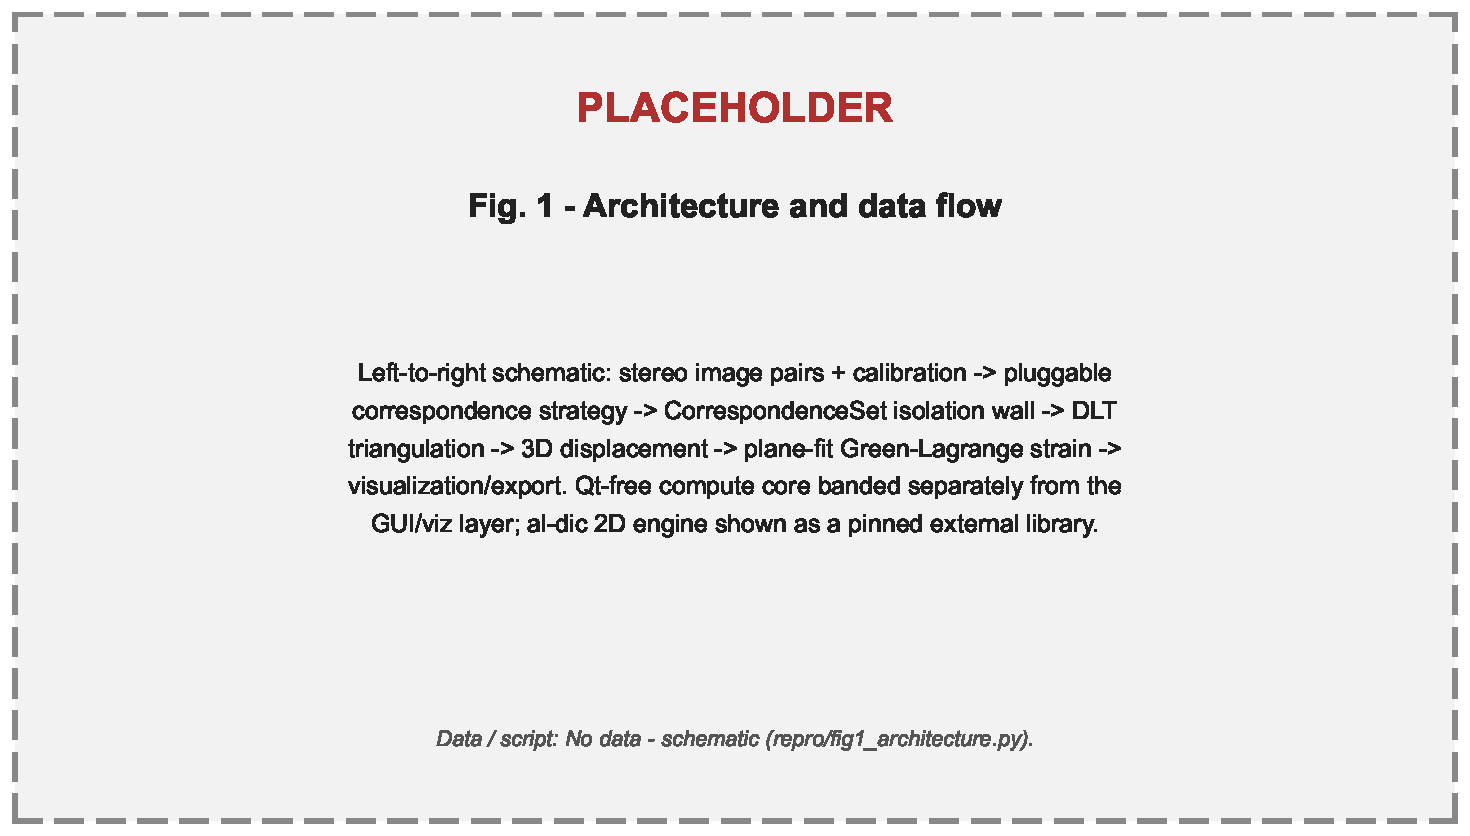
\includegraphics[width=0.92\linewidth]{figs/fig1_architecture.pdf}
\caption{pyALDIC-3D architecture and data flow. Stereo image pairs and a calibration enter at the left; \texttt{matching} resolves correspondence through one of three interchangeable strategies and emits a single \texttt{CorrespondenceSet}. That object is an isolation wall: \texttt{reconstruct}, \texttt{strain3d}, \texttt{viz3d} and \texttt{export} consume only it, never a concrete strategy. The upper band is the Qt-free compute core, scriptable without the interface; the lower band is the desktop application. The pyALDIC 2D engine is a pinned external dependency of \texttt{matching} alone.}
\label{fig:architecture}
\end{figure}
%%%%%%%%%%%%%%%%%%%%%%%%%%%%%%%%%%%%%%%%%%%%%%%

\subsection{Software functionalities}
\label{sec:func}

\subsubsection{Stereo calibration}
\label{sec:calib}

Calibration has no 2D equivalent and is mandatory: without intrinsics and relative pose, matched pixels cannot be triangulated. pyALDIC-3D performs it internally, following Zhang's planar-target method \cite{zhang2000flexible} with a Brown--Conrady distortion model, on OpenCV \cite{bradski2000opencv}. Four board families are detected --- chessboard, ChArUco, circle grid, and a coded circular-dot target whose detector was developed for this work: three ring fiducials establish board identity and orientation so partial views index correctly, edge-clipped dots are recovered by an elliptical arc fit with sub-pixel rim refinement rather than centroided, and the projected-circle centroid bias is corrected analytically. Per-camera and stereo geometry are then solved, with an optional bundle adjustment that applies a robust per-point loss, exploits views seen by only one camera, and can optimize the board's own shape to absorb printing error; poor pairs are rejected against a user-set threshold and reported individually.

Every quantity needed to judge the result is displayed: stereo reprojection RMS and epipolar residual, baseline, pairs used versus total, image-plane coverage, board-tilt range, and the RMS change contributed by bundle adjustment. Following the iDICs position that a low reprojection residual is necessary but not sufficient \cite{idics2018gpg}, a separate \emph{verification} pass measures a board of known geometry with the finished calibration and reports the recovered pitch, scale error and plane RMS in millimetres --- a direct check on absolute metric scale (Fig.~\ref{fig:calibration}) --- and a leave-$p$-out jackknife reports how sensitive the solution is to the choice of views. An existing calibration can instead be imported in one of six formats (DICe, MatchID, MATLAB \texttt{stereoParameters}, MMC/MultiDIC, OpenCorr, OpenCV) or entered by hand; all paths normalize to the same internal rig. Throughout, the left camera defines the world frame ($\mathbf{R}=\mathbf{I}$, $\mathbf{T}=\mathbf{0}$) and the right is expressed as $\mathbf{X}_R = \mathbf{R}\mathbf{X}_L + \mathbf{T}$.

%%%%%%%%%%%%%%%%%%%%%%%%%%%%%%%%%%%%%%%%%%%%%%%
% TODO(fig2): data = the authors' real coded-target photo set (D12 validation).
% Script = tools/calib_report.py -> repro/fig2_calibration.py.
\begin{figure}[htbp]
\centering
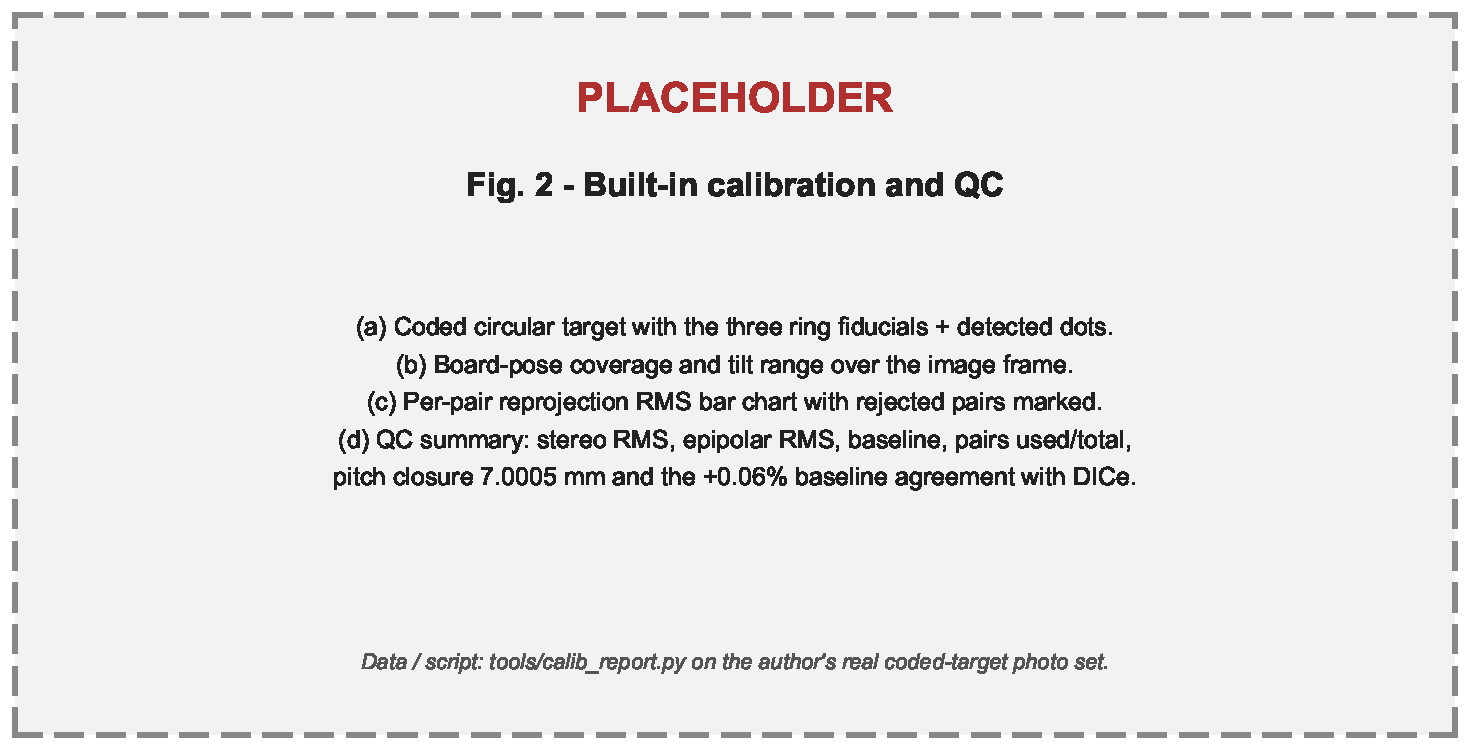
\includegraphics[width=\textwidth]{figs/fig2_calibration.pdf}
\caption{Built-in stereo calibration and its quality control. (a)~A coded circular-dot board with the three ring fiducials and all detected dot centroids overlaid. (b)~Board-pose coverage and tilt range over the image frame. (c)~Per-pair reprojection RMS, with threshold-rejected pairs marked. (d)~QC summary: stereo and epipolar RMS, baseline, pairs used/total, and the independent metric verification --- a $7$\,mm pitch recovered as $7.0005$\,mm, and a baseline within $+0.06\,\%$ of an independent DICe calibration of the same images.}
\label{fig:calibration}
\end{figure}
%%%%%%%%%%%%%%%%%%%%%%%%%%%%%%%%%%%%%%%%%%%%%%%

\subsubsection{Correspondence and 3D reconstruction}
\label{sec:corr}

Correlation runs on the \emph{raw} images; no rectification is performed, because resampling degrades the speckle. The calibrated geometry only seeds and bounds the search along the epipolar band \cite{hartley2004multiple} and supplies QC residuals; distortion is removed from point \emph{coordinates} immediately before triangulation. Temporal tracking uses the 2D engine with the Augmented Lagrangian global step on by default, coupling the local inverse-compositional Gauss--Newton subproblems through a finite-element compatibility solve \cite{yang2019augmented} over an optionally quadtree-refined mesh \cite{yang2022staq}; one switch reduces it to local DIC. Cross-camera matching is deliberately left as scattered local IC-GN, because a disparity field is projective viewpoint geometry rather than material deformation, so a displacement-compatibility regularizer does not apply --- the same choice the MATLAB reference makes.

The three shipped strategies differ in which correlations they perform, and hence in how error propagates (Fig.~\ref{fig:geometry}b). \texttt{track\_both} (default, and the strategy of the MATLAB reference) matches the cameras once on frame~1 and then tracks each independently through time: the frame-1 stereo error is a time constant that cancels to first order in the displacement, but the two temporal chains drift independently. \texttt{stereo\_each\_frame} tracks only the left camera and re-matches stereo every frame, leaving one drift chain and making the reprojection residual an honest per-frame quality signal, at the cost of fresh non-cancelling stereo noise. \texttt{ref\_direct} matches every image directly against left frame~1: drift-free, but it asks the hardest correlation --- viewpoint difference and accumulated deformation at once --- and degrades exactly when deformation is largest. Orthogonally, tracking is accumulative or incremental with a rolling reference refreshing every frame, every $N$ frames, or on a user-supplied list; increments compose as $\mathbf{U}^{k}(\mathbf{X}) = \mathbf{U}^{k-1}(\mathbf{X}) + \mathbf{u}^{k}(\mathbf{X}+\mathbf{U}^{k-1}(\mathbf{X}))$, interpolated at the \emph{deformed} position. The initial guess is an FFT integer search, a warm start, or user-placed \emph{starting points} --- redundant seeds, template-matched and propagated along mesh connectivity --- which are the reliable choice for large inter-frame motion and for multi-region ROIs where an FFT peak-picker can pick the wrong side of a discontinuity.

Given matched, undistorted normalized coordinates and the projection matrices $\mathbf{M}_L$, $\mathbf{M}_R$, the world point $\mathbf{P}$ follows from the direct linear transformation \cite{abdelaziz2015dlt}: each view contributes two constraints from $\mathbf{x}\times(\mathbf{M}\tilde{\mathbf{P}})=\mathbf{0}$, and the stacked $4\times4$ system is solved in the total least-squares sense,
%
\begin{equation}
\mathbf{A}\,\tilde{\mathbf{P}} = \mathbf{0},
\qquad
\tilde{\mathbf{P}} = \argmin_{\|\tilde{\mathbf{P}}\|=1} \|\mathbf{A}\tilde{\mathbf{P}}\|_2 ,
\label{eq:dlt}
\end{equation}
%
by singular value decomposition, followed by a reprojection-residual check. Because reconstruction returns a metric position for every node and frame, the 3D displacement is defined without reference to how correspondence was obtained,
%
\begin{equation}
\mathbf{D}^{k}(\mathbf{X}) = \mathbf{P}^{k}(\mathbf{X}) - \mathbf{P}^{1}(\mathbf{X}),
\label{eq:disp}
\end{equation}
%
which is what makes the 3D layer strategy- and mode-agnostic. Invalid nodes carry \texttt{NaN}, which propagates unchanged to the exports; all arrays are \texttt{float64} and all lengths are millimetres.

%%%%%%%%%%%%%%%%%%%%%%%%%%%%%%%%%%%%%%%%%%%%%%%
% TODO(fig3): data = none (schematic, drawn to scale from the Sample 3
% calibration). Script = repro/fig3_geometry.py.
\begin{figure}[htbp]
\centering
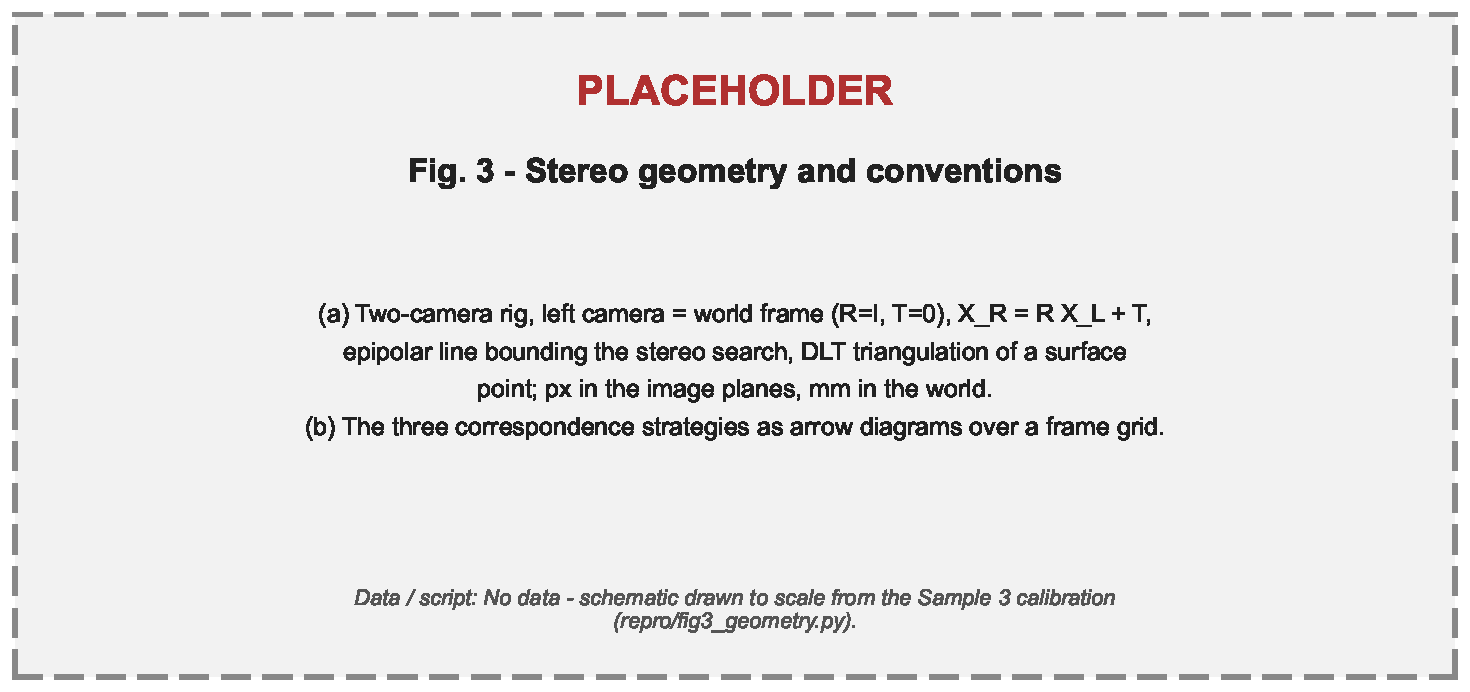
\includegraphics[width=\textwidth]{figs/fig3_geometry.pdf}
\caption{Measurement model and conventions. (a)~The rig: the left camera defines the world frame ($\mathbf{R}=\mathbf{I}$, $\mathbf{T}=\mathbf{0}$) and the right satisfies $\mathbf{X}_R=\mathbf{R}\mathbf{X}_L+\mathbf{T}$; a surface point $\mathbf{P}$ projects to $\mathbf{x}_L$ and $\mathbf{x}_R$, its epipolar line bounds the stereo search, and Eq.~\eqref{eq:dlt} recovers $\mathbf{P}$ as the least-squares ray intersection. Image planes in pixels, world in millimetres. (b)~The three correspondence strategies drawn over a sequence of frame pairs.}
\label{fig:geometry}
\end{figure}
%%%%%%%%%%%%%%%%%%%%%%%%%%%%%%%%%%%%%%%%%%%%%%%

\subsubsection{Surface strain, and crack awareness}
\label{sec:crack}

Strain is a total-Lagrangian post-process on the reconstructed point cloud, evaluated at every node on the frame-1 reference surface, following the formulation validated in the MATLAB reference \cite{tong2025stereo}. The virtual strain gauge is a square window of side $(n_{\mathrm{vsg}}-1)\Delta + 1$ pixels in the reference image ($n_{\mathrm{vsg}}$ the gauge size in grid steps, $\Delta$ the node spacing); the neighbourhood $\mathcal{N}(i)$ of node~$i$ is retrieved with a Chebyshev-metric k-d tree and must hold at least nine nodes with finite displacement. Because the surface is curved, gradients must be taken in its tangent plane rather than the camera frame: a plane $Z=aX+bY+c$ is fitted to the neighbourhood's reference positions, giving an orthonormal frame with $\hat{\mathbf{z}}\propto(a,b,-1)$. Reference coordinates and displacements are rotated into that frame and the in-plane gradients fitted by least squares, giving a gradient matrix $\mathbf{G}$ whose out-of-plane derivative row is zeroed. The deformation gradient and Green--Lagrange strain follow as
%
\begin{equation}
\mathbf{F} = \mathbf{I} + \mathbf{G}^{\!\top},
\qquad
\mathbf{E} = \tfrac{1}{2}\!\left(\mathbf{F}^{\!\top}\mathbf{F}-\mathbf{I}\right),
\label{eq:green}
\end{equation}
%
which vanishes identically under rigid-body rotation. Principal strains, maximum shear and a von Mises invariant follow from $\mathbf{E}$, with the out-of-plane slopes retained as diagnostics. Infinitesimal ($\tfrac{1}{2}(\mathbf{G}+\mathbf{G}^{\!\top})$) and Almansi ($\tfrac{1}{2}(\mathbf{I}-\mathbf{F}^{-\top}\mathbf{F}^{-1})$) measures are selectable, as are three reporting frames: the per-node tangent plane, the left-camera frame, or a specimen frame set by three picked points. Near a boundary the gauge is one-sided and biased, so nodes closer to it than $\alpha$ times the gauge radius are flagged; strain arrays stay dense and a boolean mask records what to display, so the trim can be revisited downstream.

Crack awareness reuses that machinery. With the region-of-interest cutting tools the user leaves a thin \emph{barrier} --- an excluded band --- along the discontinuity, material retained on both sides; the barrier then propagates through the whole chain automatically. It cuts the correlation mesh, so no finite element bridges the crack; it is carried into the right camera by warping the left mask through the frame-1 stereo correspondence, so both cameras are cut consistently; and it restricts each subset's correlation support to the connected component containing the subset centre, so a subset beside the crack correlates only its own face. It enters the strain gauge as a visibility test: neighbour $j$ joins $\mathcal{N}(i)$ only if the reference-configuration segment $\overline{\mathbf{X}_i\mathbf{X}_j}$ does not cross the barrier, so the plane fit of Eq.~\eqref{eq:green} is never contaminated by the far face. Finally it folds into the trim mask, so the crack band is blanked rather than filled with a fabricated value, and the interactive view, the preview and the exports blank identical cells (Fig.~\ref{fig:crack}). The result is a measured jump instead of a smoothed ramp; with no barrier present, every one of these steps is a verified no-op.

%%%%%%%%%%%%%%%%%%%%%%%%%%%%%%%%%%%%%%%%%%%%%%%
% TODO(fig4): data = a cracked-specimen stereo pair (authors' data) + two runs
% of the same session with the barrier disabled/enabled, shared colour scale.
% Script = repro/fig4_crack_aware.py.
\begin{figure}[htbp]
\centering
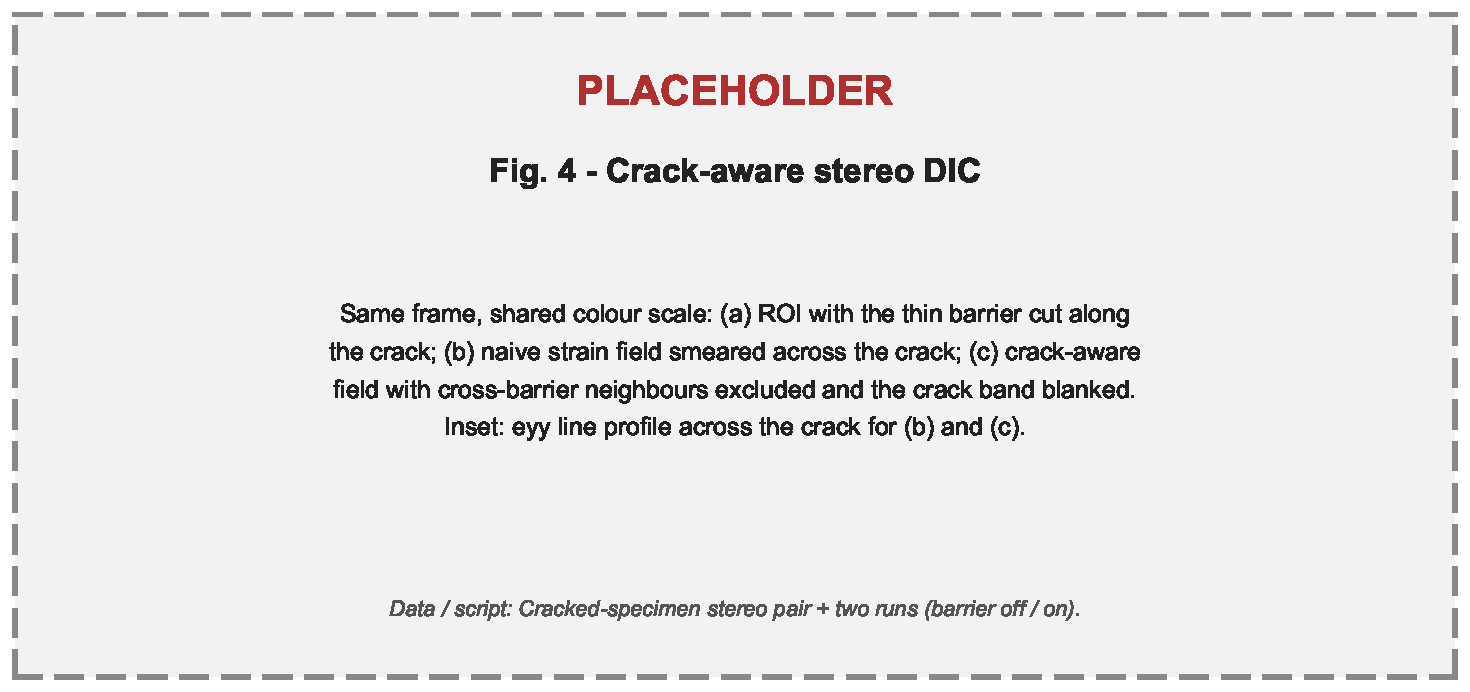
\includegraphics[width=\textwidth]{figs/fig4_crack_aware.pdf}
\caption{Crack-aware stereo DIC, all panels on a shared colour scale. (a)~The region of interest with the thin barrier cut along the crack. (b)~Naive result: an ordinary gauge neighbourhood averages both crack faces and reports a smooth ramp across the discontinuity. (c)~Crack-aware result: no neighbour pair crosses the barrier, the crack band is blanked by the trim mask, and each face carries its own strain. Inset: $\varepsilon_{yy}$ profiles perpendicular to the crack for (b) and (c), showing the jump the naive fit rounds off.}
\label{fig:crack}
\end{figure}
%%%%%%%%%%%%%%%%%%%%%%%%%%%%%%%%%%%%%%%%%%%%%%%

\subsubsection{Independent verification of the delivered field}
\label{sec:gate}

DIC solvers are engineered not to fail loudly. In the engine used here, local subsets that do not converge are replaced by inverse-distance-weighted neighbours, the global compatibility solve returns a field finite everywhere by construction, and incremental composition fills gaps by nearest neighbour. Each behaviour is defensible alone, but together they make a finiteness test on the output structurally always true: a frozen warm start, or a garbage increment faithfully composed, leaves a field that is finite, smooth and wrong. We observed exactly this during development, in both tracking modes.

pyALDIC-3D therefore re-verifies what it is about to ship, using a criterion the solver never optimized. After the temporal track returns, for every frame $k$ and node $\mathbf{X}$ the reference subset $\Omega(\mathbf{X})$ is compared with the frame-$k$ image sampled at the \emph{reported} cumulative position $\mathbf{X}+\mathbf{U}^{k}(\mathbf{X})$ under a translation warp, through the zero-normalized sum of squared differences
%
\begin{equation}
\mathrm{ZNSSD}_k(\mathbf{X}) \;=\;
\sum_{\mathbf{s}\in\Omega}
\left(
\frac{f(\mathbf{X}+\mathbf{s})-\bar{f}}{\Delta f}
-
\frac{g_k(\mathbf{X}+\mathbf{U}^{k}(\mathbf{X})+\mathbf{s})-\bar{g}_k}{\Delta g_k}
\right)^{\!2},
\label{eq:znssd}
\end{equation}
%
where $\bar{\cdot}$ and $\Delta$ denote the subset mean and the root of the summed squared deviation. The measure lies in $[0,4]$ and is invariant to affine illumination changes; the default rejection threshold of $1.0$ corresponds to a zero-normalized cross-correlation of $0.5$. Nodes above it are invalidated and --- crucially --- \emph{counted}: node-frames removed per camera, the per-frame validity fraction, the frame-1 stereo yield and the counts removed by each optional quality gate all reach the run log and the saved session, so a run that returns few points explains why (Fig.~\ref{fig:honesty}). This is an independent measurement of the delivered product, not a restatement of the solver's residual. Because it visits every node of every frame it is a substantial part of the wall time on long sequences; the kernel is Numba-compiled and chunked, giving a $3.29\times$ speedup in v1.1.0 with bit-identical verdicts (maximum absolute difference $0$ over $275{,}184$ values).

%%%%%%%%%%%%%%%%%%%%%%%%%%%%%%%%%%%%%%%%%%%%%%%
% TODO(fig5): data = tools/matlab_parity.py P2 gate output + a deliberately
% frozen-warm-start run reproducing the historical silent failure.
% Script = repro/fig5_honesty_gate.py.
\begin{figure}[htbp]
\centering
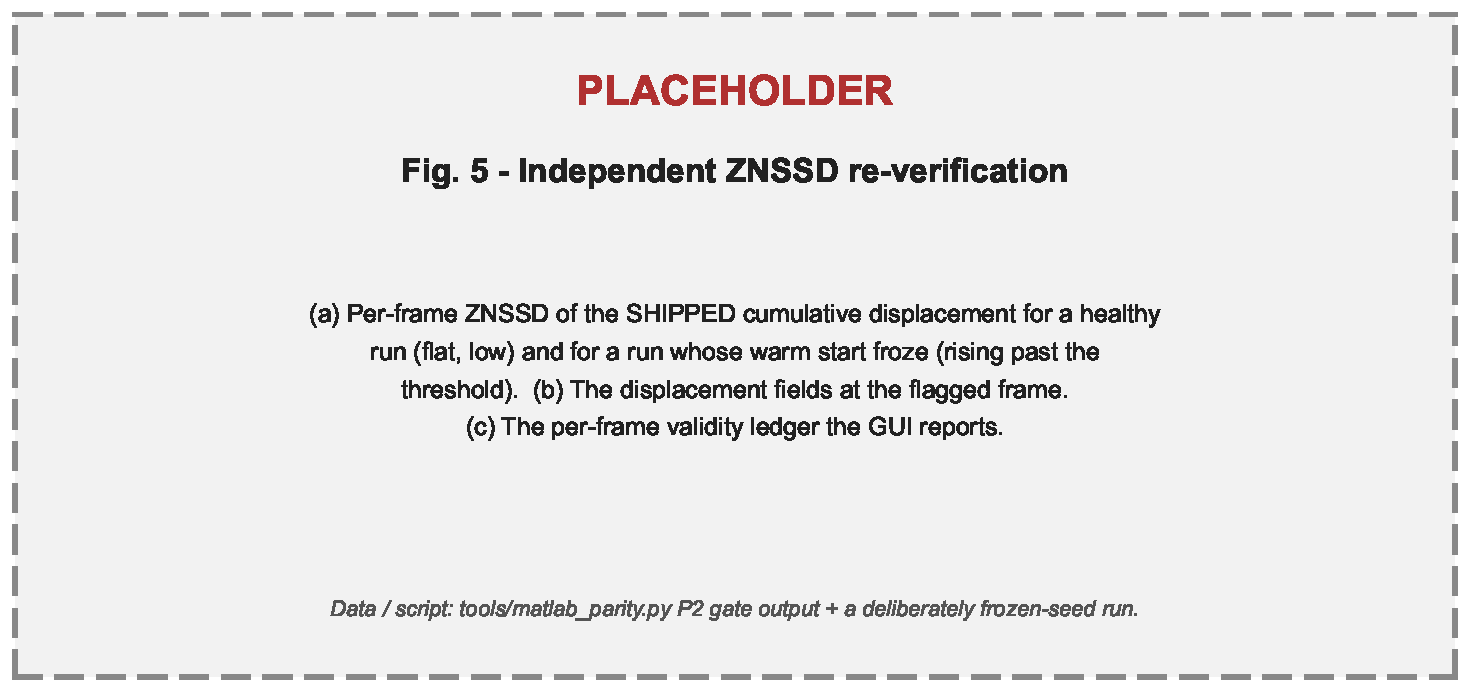
\includegraphics[width=\textwidth]{figs/fig5_honesty_gate.pdf}
\caption{Independent re-verification catching a silent solver failure. (a)~Per-frame ZNSSD of the \emph{shipped} cumulative displacement, Eq.~\eqref{eq:znssd}, for two runs on the same data: the healthy run stays flat and low, while a run whose warm start froze rises past the rejection threshold (dashed) from the marked frame onward. (b)~The displacement fields at that frame --- the frozen run is finite, smooth and entirely plausible, which is why a finiteness test misses it. (c)~The per-frame validity ledger reported to the user.}
\label{fig:honesty}
\end{figure}
%%%%%%%%%%%%%%%%%%%%%%%%%%%%%%%%%%%%%%%%%%%%%%%

\subsubsection{Interface, sessions and distribution}
\label{sec:gui}

The desktop application (Fig.~\ref{fig:gui}), launched with \texttt{al-dic-3d gui}, has three columns: a left sidebar carrying the workflow top to bottom (paired image drop zones, calibration, workflow type, initial guess, region of interest, parameters, and an advanced section exposing the correspondence strategy); a central zoom/pan canvas showing either camera with ROI, mesh, seed and result overlays; and a right sidebar with run controls, progress, field and colormap selection, physical units, the interactive 3D view, and a filterable console log. Strain post-processing runs in its own window with independent visualization state, so gauge size, strain measure and reporting frame can be explored without recomputing correspondence. Cancelling is non-destructive: computed frames are kept and later frames left \texttt{NaN}.

An entire project --- image paths, calibration, ROI and masks including the crack barrier, seeds, parameters, results and strain --- persists to a single \texttt{.aldic3d} file and reopens without recomputation. Exports cover NumPy \texttt{.npz}, MATLAB \texttt{.mat}, per-frame CSV, PLY point clouds and a VTU/PVD series for ParaView, plus images, MP4/GIF animations and offscreen 3D renders, always with a parameters JSON. Strings are translated into eight locales. The same functionality is available headless (\texttt{al-dic-3d run config.toml}, \texttt{al-dic-3d calibrate}); distribution is via PyPI, GitHub release wheels, and a standalone Windows installer needing no Python.

%%%%%%%%%%%%%%%%%%%%%%%%%%%%%%%%%%%%%%%%%%%%%%%
% TODO(fig6): data = examples/Images_Stereo_Sample3_images or the authors'
% tension dataset. Script = tools/gui_screenshot.py (offscreen, QT_QPA_FONTDIR
% set) + repro/fig6_gui.py for annotations. Capture at high DPI: all UI text
% must be legible at print size.
\begin{figure}[t!]
\centering
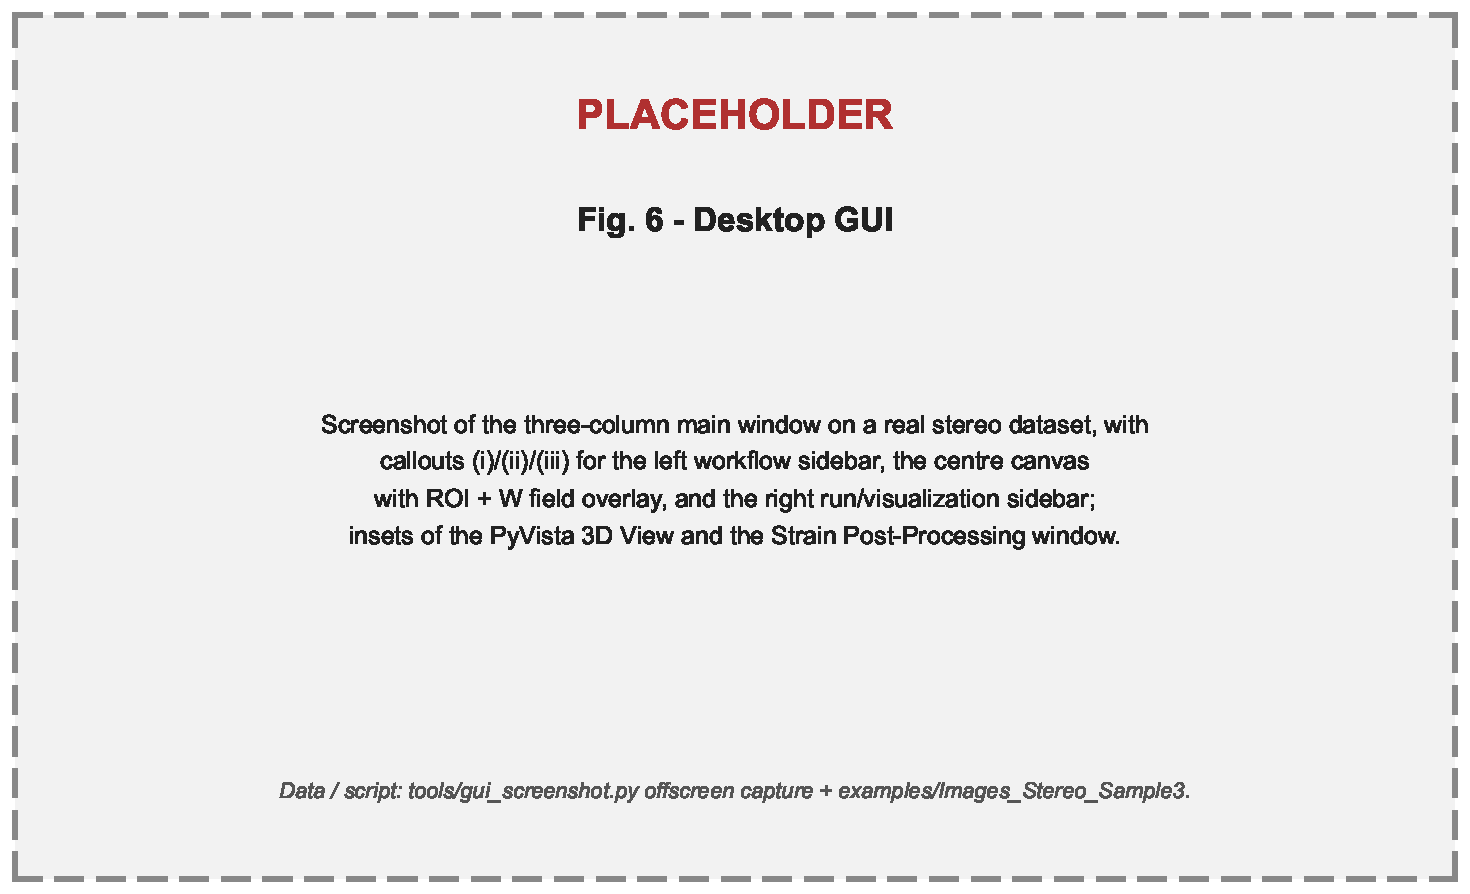
\includegraphics[width=\textwidth]{figs/fig6_gui.pdf}
\caption{The pyALDIC-3D desktop application after a stereo analysis. \textbf{(i)}~Left sidebar: the workflow in order --- paired left/right image drop zones, calibration, workflow type, initial guess, region of interest, parameters, and the advanced panel exposing the correspondence strategy. \textbf{(ii)}~Central canvas: the specimen with the region of interest and the colour-mapped out-of-plane displacement $W$. \textbf{(iii)}~Right sidebar: run controls, progress, field and colormap selection, units, the 3D view launcher, and the console log carrying the validity ledger of Section~\ref{sec:gate}. Insets: the interactive 3D view and the strain post-processing window.}
\label{fig:gui}
\end{figure}
%%%%%%%%%%%%%%%%%%%%%%%%%%%%%%%%%%%%%%%%%%%%%%%

% =======================================================
\section{Illustrative examples}
\label{sec:examples}
% =======================================================

\subsection{Agreement with the MATLAB reference implementation}

The first requirement of a port is that it reproduces the implementation whose mathematics it adopts. On Sample~3 of the Stereo-DIC Challenge \cite{ahmad2024stereochallenge,idics_challenge_site} --- a curved D-shaped coupon at $1920\times1200$ px --- the frame~$0\!\rightarrow\!1$ node-wise agreement with the published MATLAB 3D-Stereo-ALDIC implementation \cite{tong2025stereo} is a median $|{\rm difference}|$ of $1.3\,\upmu$m in $U$, $1.0\,\upmu$m in $V$ and $6.0\,\upmu$m in $W$, at regression slopes $\approx\!1.0$; the reconstructed shape agrees to $29.7\,\upmu$m in $Z$ (Fig.~\ref{fig:validation}). The larger out-of-plane figures are expected, since triangulation amplifies image-plane error along the depth direction by roughly $1/\sin\theta$ for stereo angle $\theta$ \cite{reu2013stereorig4,balcaen2017stereodic}. A second gate checks the incremental machinery against a template-matching ground truth rather than against the other code, and closes at $0.38$ and $0.43$\,px.

\subsection{Community benchmarks}

On Stereo-DIC Challenge~1.0 material \cite{ahmad2024stereochallenge}, a rigid-translation set with exact ground truth is recovered to a median $0.1$--$0.3\,\upmu$m over $16$ steps; a simulated tension sequence agrees with a MatchID analysis of the same images to $0.5\,\upmu$m along the loading axis; and a real tension-to-fracture sequence runs end to end to $10.9\,\%$ strain with $98\,\%$ of nodes still valid, at a strain noise floor of $12\,\upmu\varepsilon$. On DIC Challenge~2.0 Task~1 \cite{reu2022dicchallenge2}, displacements agree with DICe to a median $0.003$--$0.015$\,px over $11{,}300$ points per frame, and the axial strain at the reference station is $0.269\,\%$ against the published $0.26\,\%$ anchor. The built-in calibrator was separately validated on a physical coded target: stereo reprojection RMS $0.293$\,px, a baseline within $+0.06\,\%$ of a DICe calibration of the same photographs, and triangulated point spacing closing at $7.0005 \pm 0.0010$\,mm against a nominal $7$\,mm.

%%%%%%%%%%%%%%%%%%%%%%%%%%%%%%%%%%%%%%%%%%%%%%%
% TODO(fig7): data = tools/matlab_parity.py (P1 gate), tools/challenge_c2_task1.py,
% tools/challenge_s2.py, tools/challenge_s4.py. Script = repro/fig7_validation.py.
\begin{figure}[t!]
\centering
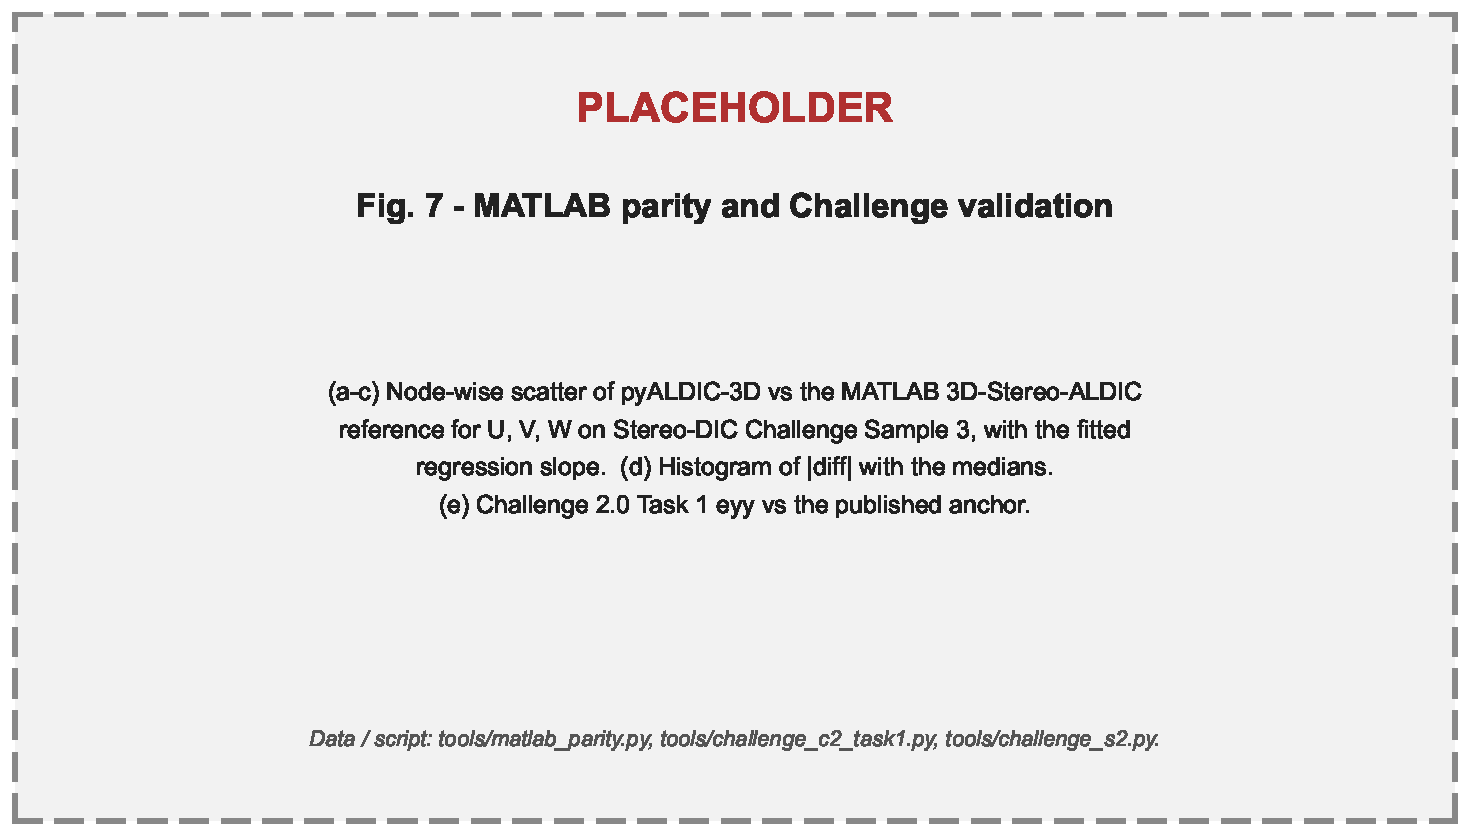
\includegraphics[width=\textwidth]{figs/fig7_validation.pdf}
\caption{Validation. (a--c)~Node-wise comparison against the MATLAB 3D-Stereo-ALDIC reference \cite{tong2025stereo} on Stereo-DIC Challenge Sample~3, frame $0\!\rightarrow\!1$, for $U$, $V$ and $W$, with the $1{:}1$ line and fitted slope. (d)~Histograms of the node-wise absolute difference (medians $1.3$, $1.0$, $6.0\,\upmu$m). (e)~DIC Challenge~2.0 Task~1: recovered axial strain against the published anchor.}
\label{fig:validation}
\end{figure}
%%%%%%%%%%%%%%%%%%%%%%%%%%%%%%%%%%%%%%%%%%%%%%%

\subsection{Scale, accuracy over long sequences, and performance}

Experimental campaigns produce long sequences at full sensor resolution, where naive implementations exhaust memory or accumulate drift. Two stress runs on synthetic data with known ground truth characterize the limits (Table~\ref{tab:perf}, Fig.~\ref{fig:scale}). A $150$-frame sequence of $12$\,Mpx pairs ($27{,}170$ nodes) completes in $58.9$\,min at a peak resident set of $5.68$\,GB, close to the $4.63$\,GB projected beforehand by the fail-fast memory check; images are streamed lazily rather than held, so memory is governed by the mesh and working set, not by sequence length. A $400$-frame sequence of $5$\,Mpx pairs ($11{,}466$ nodes) completes in $48.4$\,min at a median $1.02$\,s per frame with $100\,\%$ node validity, and --- the point of the test --- the end-frame accuracy against ground truth is $0.011$\,px in the image plane and $0.0039$\,mm in 3D, with no drift. On top of NumPy and SciPy \cite{harris2020numpy,virtanen2020scipy}, the two heaviest kernels are compiled by Numba \cite{lam2015numba}: the strain kernel is $6.5$--$19\times$ faster than the array reference (agreement below $10^{-9}$), the verification kernel $3.29\times$ faster with bit-identical verdicts.

%%%%%%%%%%%%%%%%%%%%%%%%%%%%%%%%%%%%%%%%%%%%%%%%%%
\begin{table}[htbp]
\centering
\caption{Scale tests on synthetic stereo sequences with known ground truth. ``End-frame error'' is measured against the synthetic ground truth at the last frame and shows no growth with sequence length.}
\label{tab:perf}
\begin{tabular}{lcc}
\toprule
 & $150$ frames $\times$ $12$\,Mpx & $400$ frames $\times$ $5$\,Mpx \\
\midrule
Nodes                        & $27{,}170$ & $11{,}466$ \\
Wall time                    & $58.9$ min & $48.4$ min \\
Median tracking time / frame & ---        & $1.02$ s \\
Peak resident memory         & $5.68$ GB  & $3.06$ GB \\
Node validity                & $100\,\%$  & $100\,\%$ \\
End-frame error, image plane & $0.010$ px & $0.011$ px \\
End-frame error, 3D point    & $0.002$ mm & $0.0039$ mm \\
\bottomrule
\end{tabular}
\end{table}
%%%%%%%%%%%%%%%%%%%%%%%%%%%%%%%%%%%%%%%%%%%%%%%%%%

%%%%%%%%%%%%%%%%%%%%%%%%%%%%%%%%%%%%%%%%%%%%%%%
% TODO(fig8): data = tools/stress_synth.py logs (G4) + tools/bench_strain3d.py.
% Script = repro/fig8_scale.py. Candidate for merging into Fig. 7 (6-fig cap).
\begin{figure}[htbp]
\centering
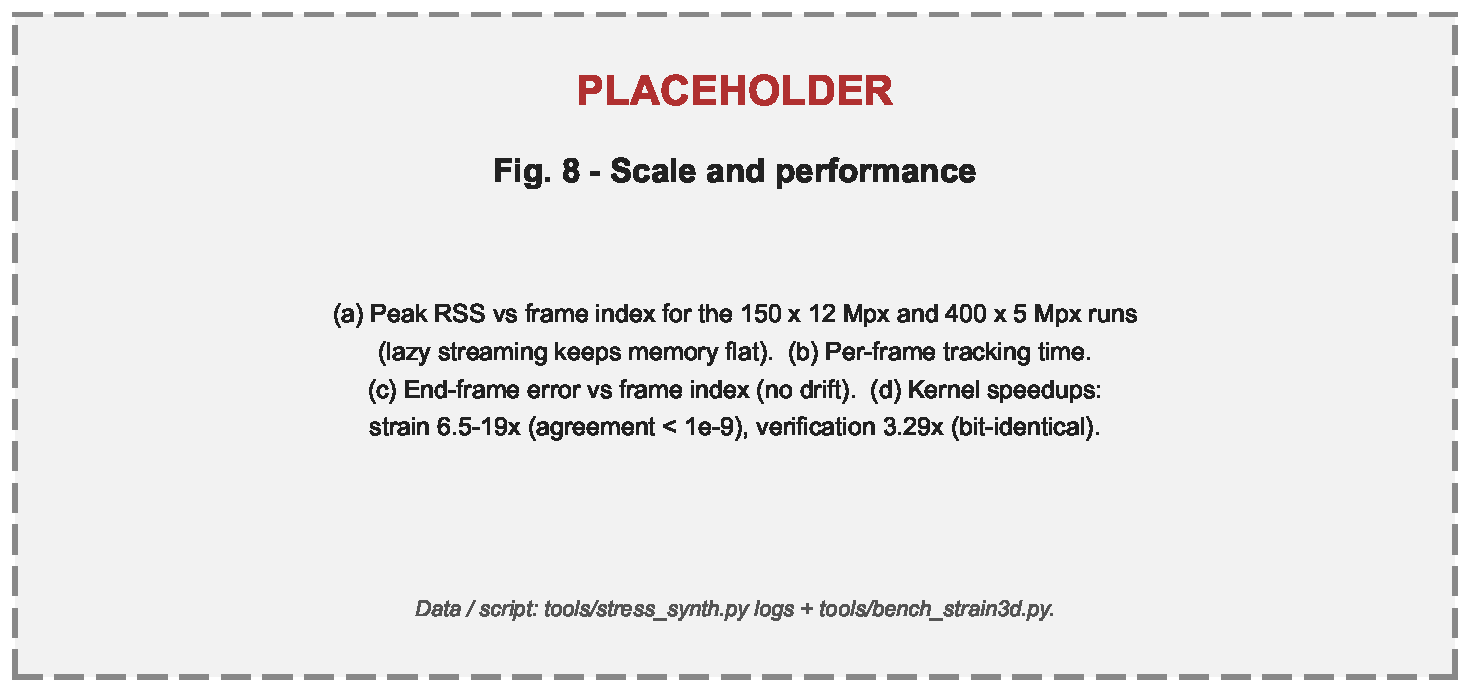
\includegraphics[width=\textwidth]{figs/fig8_scale.pdf}
\caption{Scale and performance. (a)~Resident memory against frame index for the two runs of Table~\ref{tab:perf}: lazy streaming keeps memory flat rather than growing with sequence length. (b)~Per-frame tracking time over the $400$-frame run, showing no degradation. (c)~Error against the synthetic ground truth versus frame index, demonstrating the absence of drift. (d)~Numba kernel speedups: $6.5$--$19\times$ (strain) and $3.29\times$ (verification).}
\label{fig:scale}
\end{figure}
%%%%%%%%%%%%%%%%%%%%%%%%%%%%%%%%%%%%%%%%%%%%%%%

% =======================================================
\section{Impact and conclusions}
\label{sec:impact}
% =======================================================

\paragraph{Removing the barriers to stereo-DIC} Stereo-DIC has been practically gated behind either a commercial license or a MATLAB license plus a chain of separate tools. pyALDIC-3D delivers the complete chain --- calibration, correspondence, reconstruction, finite surface strain, visualization and export --- as one BSD-3-Clause application that installs with a single command on Windows, macOS and Linux, or from a double-clickable installer for users with no Python at all. Because the core is Qt-free, the identical pipeline runs headless, so exploratory work and batch reprocessing share one implementation and one result format.

\paragraph{A position on trustworthy DIC software} The verification gate of Section~\ref{sec:gate} is a methodological point rather than a feature. Full-field measurement software returns dense arrays of plausible numbers whether or not the underlying correlations succeeded, and the usual defences --- correlation residual, convergence flag, finiteness --- are all statements the solver makes about itself. We argue that a measurement tool should additionally re-measure its own deliverable against a criterion it did not optimize, and account for every point it discards. Doing so cost one pass over the data and caught failures that would otherwise have been published; we recommend the practice to other DIC implementations.

\paragraph{Standards alignment and provenance} Parameter naming, region-of-interest conventions, calibration QC reporting and strain-gauge terminology follow the iDICs \emph{Good Practices Guide} \cite{idics2018gpg,idics2025gpg}. The underlying algorithms are community-validated: AL-DIC \cite{yang2019augmented} was assessed in DIC Challenge~2.0 \cite{reu2022dicchallenge2} and extended to volumetric \cite{yang2020augmented} and stereo \cite{tong2025stereo} settings, and this implementation is checked directly against that stereo reference.

\paragraph{Conclusions and roadmap} pyALDIC-3D is an open-source, cross-platform, GUI-based stereo-DIC application spanning calibration through 3D surface strain, with pluggable correspondence strategies, crack-aware handling of discontinuous fields and independent verification of its own output. It agrees with the published MATLAB reference to $1.3$/$1.0$/$6.0\,\upmu$m in $U$/$V$/$W$ and with community benchmarks at the sub-pixel level, and sustains $400$-frame sequences without drift. The roadmap targets $N$-camera rigs, a quality-driven adaptive correspondence strategy that re-anchors on demand and rescues lost points, and GPU acceleration. Source code, documentation and worked examples are openly available at \url{https://github.com/zachtong/pyALDIC-3D}.

% =======================================================
\section*{CRediT authorship contribution statement}
% =======================================================
\textbf{Zixiang Tong:} Conceptualization, Methodology, Software, Validation, Formal analysis, Investigation, Data curation, Visualization, Writing -- original draft, Writing -- review \& editing. \textbf{Jin Yang:} Conceptualization, Methodology, Supervision, Resources, Funding acquisition, Project administration, Writing -- review \& editing.

% =======================================================
\section*{Conflict of interest}
% =======================================================
The authors declare no conflict of interest. There has been no significant financial support for this work that could have influenced its outcome.

% =======================================================
\section*{Data availability}
% =======================================================
Runnable worked examples, their configuration files and the scripts that regenerate every reported figure are distributed with the source repository and archived on Zenodo \cite{pyaldic3d_zenodo}. The Stereo-DIC Challenge and DIC Challenge~2.0 materials used for validation are distributed by the International Digital Image Correlation Society \cite{idics_challenge_site}. Experimental images acquired by the authors are released under the same license as the code.

% =======================================================
\section*{Declaration of generative AI and AI-assisted technologies in the manuscript preparation process}
% =======================================================
During the preparation of this work the authors used Anthropic Claude to polish manuscript text, to generate schematic explanatory figures via matplotlib code, and to format LaTeX tables. After using this tool, the authors reviewed and edited the content as needed and take full responsibility for the content of the publication.

% =======================================================
\section*{Acknowledgements}
% =======================================================
Z.T. thanks the University Graduate Continuing Fellowship, the Graduate Excellence Fellowship, and the Professional Development Award from the University of Texas at Austin Cockrell School of Engineering. J.Y. gratefully acknowledges support from the U.S. National Science Foundation (NSF) under Grants No. 2232428, 2441460, and 2452029, and the Pilot Seed Gift from the Semiconductor Research Corporation.

% =======================================================
% References
% =======================================================
\bibliographystyle{elsarticle-num}
\bibliography{reference}

\end{document}
\endinput
